\graphicspath{{Images/}}

\section{Ejercicio 4}

\subsection{Consigna}

Escribir un programa que dado el archivo \emph{homo\_sapiens\_chromosome\_1.fasta}, lo particione en \textbf{n} partes (donde \textbf{n} es el número total del procesadores), envíe cada una de esas porciones a los respectivos procesos y busque la cantidad de veces que aparece la base A (adenina), devolviendo al master la cantidad de veces que cada proceso contabilizó. Finalmente calcule el porcentaje de A en el cromosoma.

\subsection{Resolución}
\subsubsection{Implementación con MPI}

\lstinputlisting[language=C++]{codigos/main4.cpp}


\subsubsection{Ejecución}
Para compilar el código propuesto utilicé el comando:
\begin{lstlisting}
    mpicxx.mpich -o main.bin main.cpp
\end{lstlisting}

Habiendo compilado el código procedí a correrlo con el siguiente comando:

\begin{lstlisting}
    mpiexec.mpich -n n ./main.bin
\end{lstlisting}

\hspace{5mm} Siendo \textit{n} el número de procesos.

Tras finalizada su ejecución, la salida se guarda con formato csv para que luego sea facilmente manipulado con la libreria pandas.

\subsubsection{Análisis}

%insertar análisis%
Habiendo obtenido el número de ocurrencias procedí a cargar los datos a un DataFrame(\ref{fig:dfej4}) de la librería pandas \cite{noauthor_pandasdataframe_nodate}. Allí generé gráficas de barra con el número de ocurrencias para cada una de las bases (\ref{fig:grafica1ej4}). Luego realicé el cálculo de los porcentajes y, de la misma forma que las ocurrencias, las visualicé (\ref{fig:grafica2ej4}).



% \begin{figure}[H]
%     \centering
%     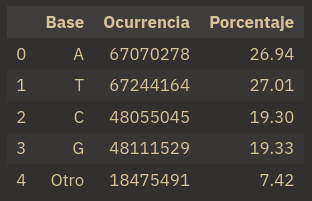
\includegraphics[width=0.35\textwidth]{Images/Captura desde 2023-08-29 18-54-27.png}
%     % \caption{DataFrame obtenido tras la carga de datos}
%     % \label{fig:dfej4}
% \end{figure}


\begin{table}[h!]
\centering
 \begin{tabular}{|c c c|} 
 \hline
        Base &  Ocurrencia &  Porcentaje \\
        \hline
        A &    67070278 &       26.94 \\
        \hline
        T &    67244164 &       27.01 \\
        \hline
        C &    48055045 &       19.30 \\
        \hline
        G &    48111529 &       19.33 \\
        \hline
        Otro &    18475491 &        7.42 \\
 \hline
 \end{tabular}
 \caption{DataFrame obtenido tras la carga de datos}
\label{fig:dfej4}
\end{table}

\begin{figure}[H]
    \centering
    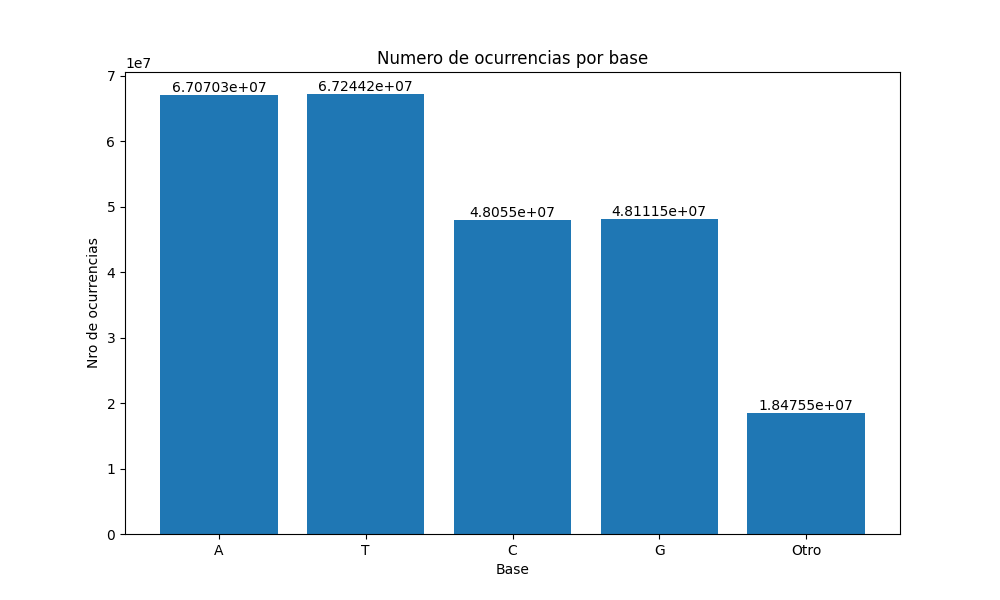
\includegraphics[width=0.70\textwidth]{Images/fig1.png}
    \caption{Gráfico de barra del número de ocurrencia por base}
    \label{fig:grafica1ej4}
\end{figure}

\begin{figure}[H]
    \centering
    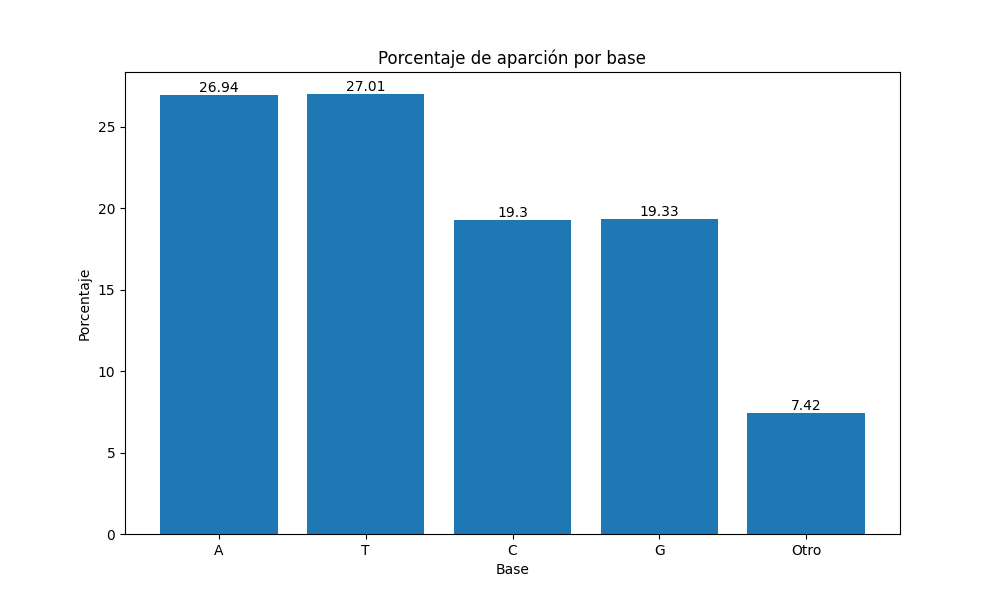
\includegraphics[width=0.70\textwidth]{Images/fig2.png}   
    \caption{Gráfico de barra del porcentaje de aparición de cada base}
    \label{fig:grafica2ej4}
\end{figure}

Por otro lado, decidí comprobar los resultados obtenidos con un script de bash. En él conte el número de ocurrencias con utilidades propias de este interpreté y obtuve los mismos resultados.

%insertar codigo%
El script mencionado es el siguiente:
% \begin{lstlisting}
% #!/bin/bash
% ocurrencias=$(grep -o "A" data/*fasta | wc -l)
% echo "El número de ocurrencias de A es: $ocurrencias"

% ocurrencias=$(grep -o "T" data/*fasta | wc -l)
% echo "El número de ocurrencias de T es: $ocurrencias"

% ocurrencias=$(grep -o "G" data/*fasta | wc -l)
% echo "El número de ocurrencias de G es: $ocurrencias"

% ocurrencias=$(grep -o "C" data/*fasta | wc -l)
% echo "El número de ocurrencias de C es: $ocurrencias"
% \end{lstlisting}

\begin{figure}[H]
    \centering
    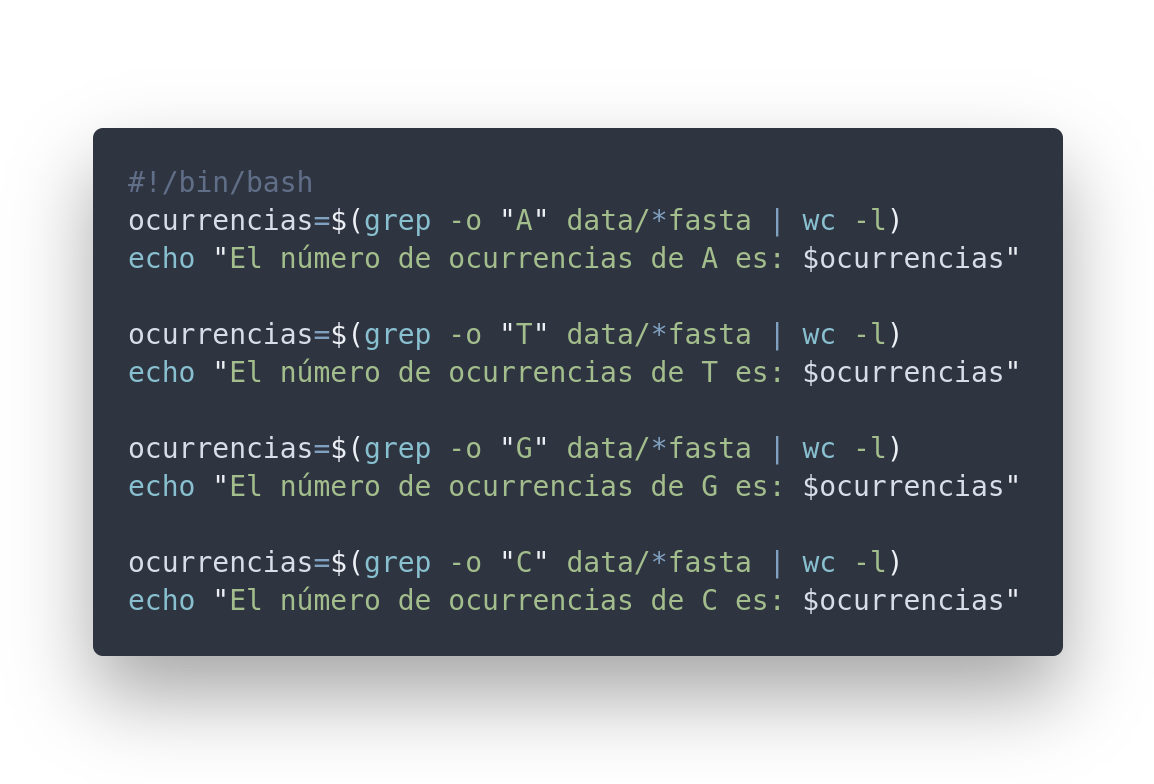
\includegraphics[width=0.70\textwidth]{Images/ej4/script.png}
    \caption{Script implementado}
    \label{fig:scriptej4}
\end{figure}

Tras ejecutarlo, obtuve la siguiente salida (\ref{fig:salidaej4}), que como se puede apreciar, concuerda con los datos obtenidos del procesamiento en paralelo con MPI:



\begin{figure}[H]
    \centering
    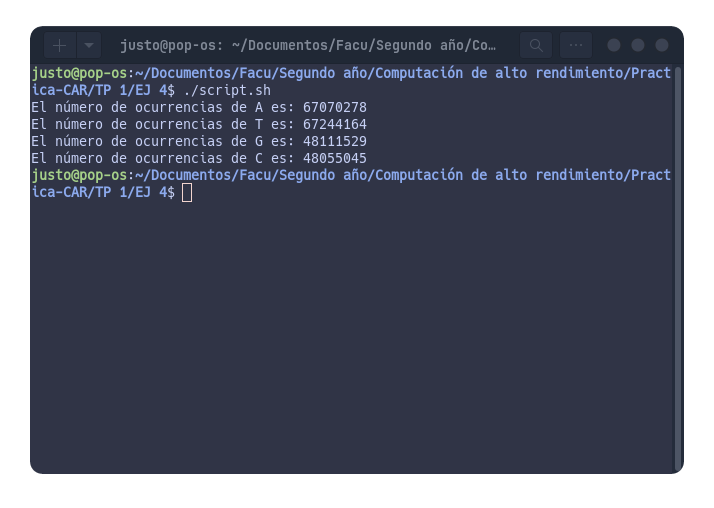
\includegraphics[width=0.80\textwidth]{Images/Captura desde 2023-08-29 16-57-42.png}
    \caption{Salida obtenida de script.sh}
    \label{fig:salidaej4}
\end{figure}